\documentclass{article}

\usepackage{tikz}
\usepackage{stanli}
\usepackage{tikzcivil}

\usetikzlibrary{decorations.pathreplacing}
\tikzset{%
  show curve controls/.style={
    postaction={
      decoration={
        show path construction,
        curveto code={
          \draw [blue] 
            (\tikzinputsegmentfirst) -- (\tikzinputsegmentsupporta)
            (\tikzinputsegmentlast) -- (\tikzinputsegmentsupportb);
          \fill [red, opacity=0.5] 
            (\tikzinputsegmentsupporta) circle [radius=.5ex]
            (\tikzinputsegmentsupportb) circle [radius=.5ex];
        }
      },
      decorate
}}}

\begin{document}
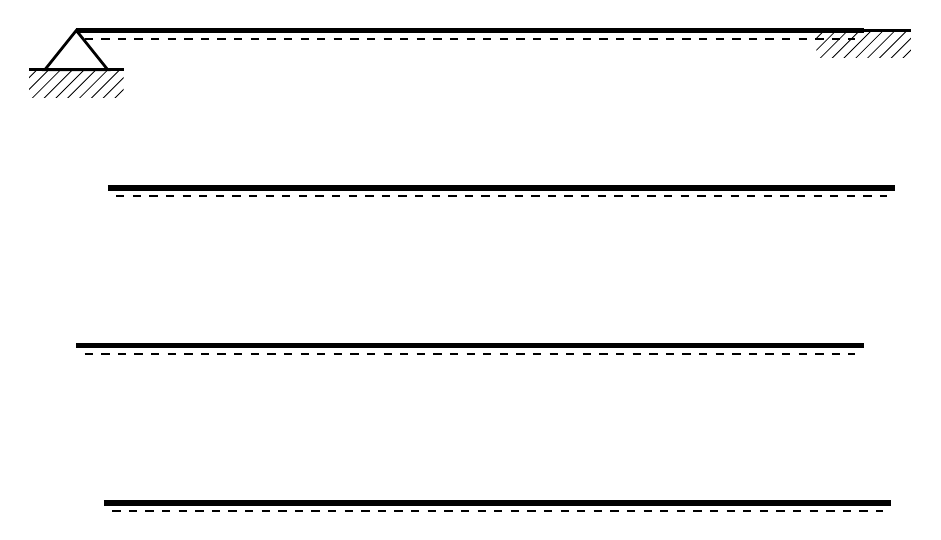
\begin{tikzpicture}

	\scaling{1}
	
	% Nodes
	% label, x, y
	\point{A}{0}{0}
	\point{B}{10}{0}

	
	% Element
	% , SN, EN
	\beam{1}{A}{B}
	
	% Fixity
	% Type, Node, angle of support (deg)
	% 1: pin
	% 2: roller
	% 3: fixed
	% 4: wall roller
	% 5: spring
	% 6: rotational spring
	\support{1}{A}{90}
	\support{3}{B}{32}
	%\Support[position={10,0}, angle=90, width = 1cm, type=fixedsliding]
%	\Support[position=A, angle=-90, width=1cm, type=fixed]
	
	%\axisTwo[position={-2,0}]{$\vec{e_1}$}{$\vec{e_2}$}

% Label DoF
\axisTwoRot[position={0cm, 1cm}]{1}{2}{3}
\axisTwoRot[position={10cm, 1cm}]{4}{5}{6}



	
	% Nodes
	% label, x, y
	\point{A}{0.4}{-2}
	\point{B}{10.4}{-2}

	
	% Element
	% , SN, EN
	\beam{1}{A}{B}
	
	% Fixity
	% Type, Node, angle of support (deg)
	% 1: pin
	% 2: roller
	% 3: fixed
	% 4: wall roller
	% 5: spring
	% 6: rotational spring
	\Support[position=A, angle=-90,
width = 1cm, type=fixedsliding]
	\Support[position=B, angle=90, width=1cm, type=fixed]
	
	%\axisTwo[position={-2,0}]{$\vec{e_1}$}{$\vec{e_2}$}

% Label DoF
%\axisTwoRot[position={0cm, 1cm}]{1}{2}{3}
%\axisTwoRot[position={10cm, 1cm}]{4}{5}{6}

	
	% Nodes
	% label, x, y
	\point{A}{0}{-4}
	\point{B}{10}{-4}

	
	% Element
	% , SN, EN
	\beam{1}{A}{B}
	
	% Fixity
	% Type, Node, angle of support (deg)
	% 1: pin
	% 2: roller
	% 3: fixed
	% 4: wall roller
	% 5: spring
	% 6: rotational spring
	\Support[position=A, angle=-90,
width = 1cm, type=fixed]
	\Support[position=B, angle=90, width=1cm, type=pinned]
	
	%\axisTwo[position={-2,0}]{$\vec{e_1}$}{$\vec{e_2}$}

% Label DoF
%\axisTwoRot[position={0cm, 1cm}]{1}{2}{3}
%\axisTwoRot[position={10cm, 1cm}]{4}{5}{6}

	
	% Nodes
	% label, x, y
	\point{A}{0.35}{-6}
	\point{B}{10.35}{-6}

	
	% Element
	% , SN, EN
	\beam{1}{A}{B}
	
	% Fixity
	% Type, Node, angle of support (deg)
	% 1: pin
	% 2: roller
	% 3: fixed
	% 4: wall roller
	% 5: spring
	% 6: rotational spring
	\Support[position=A, angle=-90,
width = 1cm, type=pinned]
	\Support[position=B, angle=90, width=1cm, type=fixed]
	
	%\axisTwo[position={-2,0}]{$\vec{e_1}$}{$\vec{e_2}$}

% Label DoF
%\axisTwoRot[position={0cm, 1cm}]{1}{2}{3}
%\axisTwoRot[position={10cm, 1cm}]{4}{5}{6}

\end{tikzpicture}
	
\end{document}
